\documentclass[11pt, a4paper]{article}
\usepackage[utf8]{inputenc} 
\usepackage{fullpage}
\usepackage{graphicx}
\usepackage[hidelinks]{hyperref,xcolor}
\usepackage[left=0.5in, right=0.5in, top=0.5in, bottom=0.5in]{geometry}
\usepackage{tocbibind} % This package automatically adds bibliography to TOC
\usepackage{float}
\renewcommand\UrlFont{\color{blue}\rmfamily}

% Bibliography management
%  see https://www.overleaf.com/learn/latex/Biblatex_citation_styles
%  and https://www.overleaf.com/learn/latex/Bibliography_management_in_LaTeX
% to use overleaf with reference manager
%  see: https://no.overleaf.com/blog/639-tip-of-the-week-overleaf-and-reference-managers
% \usepackage[backend=biber]{biblatex}
% \addbibresource{library.bib} %Imports bibliography file
 
% Title of your project
\title{Prediction of drug–protein binding affinity using existing graph convolutional neural network models on URV In-house dataset}

% Name of deliverable
\newcommand{\deliverableName}{MASTER’S Thesis FINAL PROJECT}

% Group names(s)
\author{Youssef Ezz Eldeen Ezzat}

% Group number
\newcommand{\groupNumber}{x}

% Any comments for us
\newcommand{\comments}{Comments for teachers of the course}

 % Web address for the project (if any)
\newcommand{\homepage}{\url{https://www.ntnu.edu/studies/courses/IT3010}}

% Date for title page, default is today
\date{\today}


\makeatletter{}

\begin{document}

% Title page based on https://www.latextemplates.com/template/academic-title-page
\begin{titlepage}

  	\newcommand{\HRule}{\rule{\linewidth}{0.3mm}} % Defines a new command for horizontal lines, change thickness here
	\center % Centre everything on the page
	%------------------------------------------------
	%	Headings
	%------------------------------------------------
	
	%------------------------------------------------
	%	Author(s)
	%------------------------------------------------

	% If you don't want a supervisor, uncomment the two lines below and comment the code above
 	%	{\large\textit{Author}}\\
	{\large\sc\@author}\\[1.5cm] % Your name

	\textsc{\LARGE MASTER’S DEGREE IN SECURITY ENGINEERING AND ARTIFICAL INTELLIGENCE (MESIIA)}\\[1.5cm]
	
	\textsc{\Large \deliverableName}\\[0.5cm]
	
	\textsc{\large Directed by Prof. Francesc Serratosa}\\[0.5cm]
	
	%------------------------------------------------
	%	Title
	%------------------------------------------------
	
	\HRule\\[0.4cm]
	
	{\huge\bfseries \@title}\\[0.4cm]
	
	\HRule\\[1.5cm]
	
	

 %   \footnotesize{Comments: \comments}
%   \vfill\vfill
%    \homepage
%    \vfill
    
    %------------------------------------------------
    % Change log for the plan (can be deleted before delivery)
    % When you update the plan please record what you changed and what the reason for the change. This will be useful for your supervisor.
    %------------------------------------------------
    % \input{./changelog.tex}
	
	%------------------------------------------------
	%	Logo
	%------------------------------------------------
	\vfill
	
\includegraphics[width=0.3\textwidth]{./urvlogo.png}\\[2.0cm]
	
	 
		
	%------------------------------------------------
	%	City
	%------------------------------------------------
	
	
	{\large Tarragona} % City

	
		
	%------------------------------------------------
	%	Date
	%------------------------------------------------
	
	{\large\@date} % Date, change the \today to a set date if you want to be precise
    \vfill
	
	
\end{titlepage}


\tableofcontents

\section{Introduction}


A virus encodes one or more proteases which are enzymes that spur the formation of new protein products, thus play crucial roles in virus replication ,
and are important targets for the design and development of potent antiviral agents or drugs.
Binding affinity is the strength of the binding interaction between a single biomolecule (e.g., a virus protein) to its ligand or binding partner (e.g., a drug).
it is a key to appreciating the intermolecular interactions driving biological processes and measured as part of the drug discovery process to help design drugs that bind their targets selectively and specifically.

The development of new drugs is costly, time consuming and often accompanied with safety issues.
Drug repurposing can avoid the expensive and lengthy process of drug development by finding new uses for already approved drugs. In order to repurpose drugs effectively, it is useful to know which proteins are targeted by
which drugs which is the definition of Drug-Target-Affinity(DTA)\cite{1}

\section{Aim}

The aim of this thesis is to make use of four existing convolutional neural network(CNN) models following the paper in \cite{1} - to take advantage of the fact that they represents drugs as graphs and use graph neural networks to predict DTA-
in order to train a neural network on a new small in-house URV dataset of sample size 332 patterns. but since the CNN models typically require large datasets for training like the datasets 
davis and kiba that have sample sizes of 30058 ( 25047 train + 5011 test ) and 118257 (98547 train + 19710 test) respectively used to train the CNN models in \cite{1} the approach taken will be:
\begin{itemize}
    \item Apply k-folding with k = 10 to get 10 different combinations of train and test patterns for URV dataset
    
    \begin{figure}[H]
        \centering
        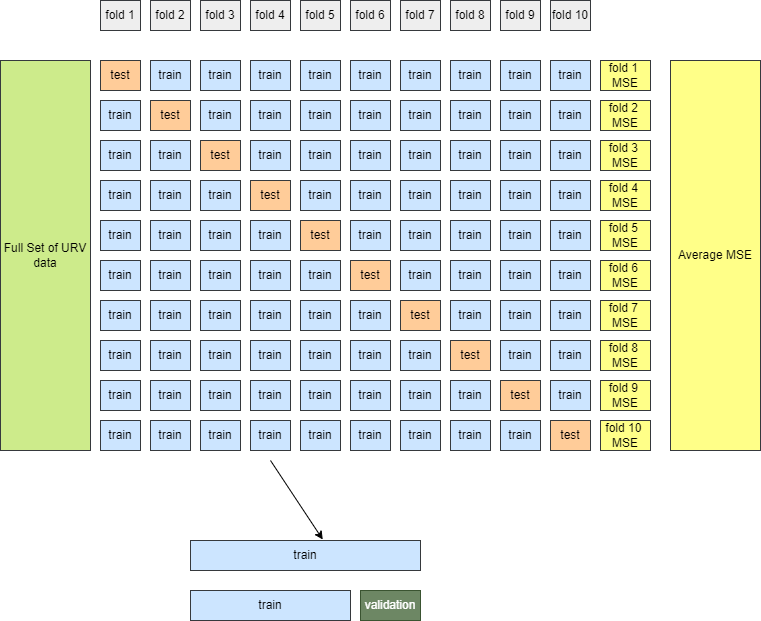
\includegraphics[scale=0.4]{Kfold.png} % Replace 'example-image' with the path to your image file
        \caption{k-folding.}
        \label{fig 1}
    \end{figure}
            
\end{itemize} 

the GIT repository of the code \cite{2} used in the referenced paper \cite{1} was forked to Git repository \cite{3} to experiment with the 
code in the referenced paper and obtain the results. code refactoring was done to run experiments in python notebooks instead of terminals

\section{URV dataset}
    \subsection{protein representation}
    the protein data are initially provided as \textbf{Protein Data Bank(PDB)} files. PDB is a file format used to store 3D structural information about proteins. It is one of the most widely used formats for representing and exchanging structural data in bioinformatics and structural biology.
    PDB files contain atomic coordinates of atoms in a molecule, along with metadata and additional information such as experimental methods used to determine the structure.

    the PDB file name is named after the protein ID. if a PDB file e.g. \textbf{6M2N\_protein.pdb}  is open with any text editor e.g. notepad++, the metadata including its ID, name, type
    are in the header and title tags as shown in figure \ref{fig 2} for protein ID \textbf{6M2N} 

        \begin{figure}[h]
            \centering
            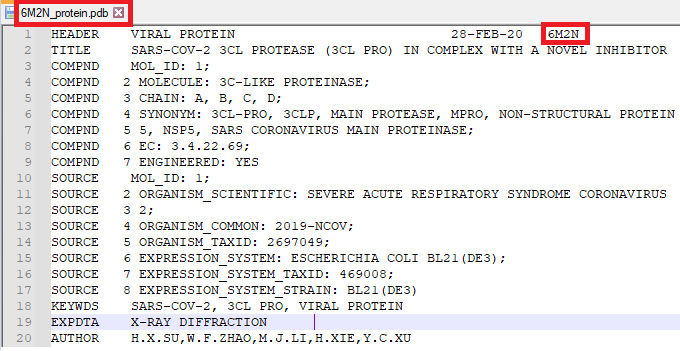
\includegraphics[width=0.75\textwidth]{pdb file.png} % Replace 'example-image' with the path to your image file
            \caption{PDB file example.}
            \label{fig 2}
        \end{figure}

    more informtion can be viewed at the PDB website \cite{4} for the same protein ID \textbf{6M2N}
        \begin{figure}[h]
            \centering
            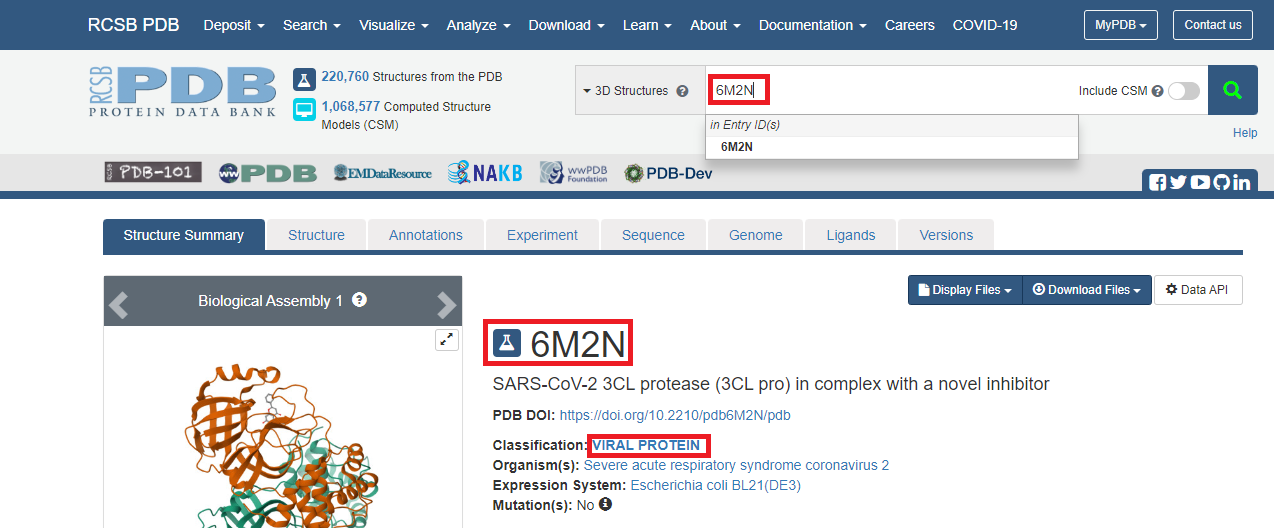
\includegraphics[width=0.75\textwidth]{pdb website.PNG} % Replace 'example-image' with the path to your image file
            \caption{PDB file example.}
            \label{fig 3}
        \end{figure}

    a protein can be either Single Chain or Multi-Chain, so it can be composed of one chain of amino acids(sequence) or more usually two, we pick the longest sequence as the representation for the protein
    this is done using \textbf{Bio.PDB} module in the \textbf{Biopython} library that provides tools for working with Protein Data Bank (PDB) files in python. classes used are:
    \begin{itemize}
        \item \textbf{PDBParser} used to parse PDB files, create a structure object and read the atomic coordinates and other structural information from a PDB file and converts it into a hierarchical structure object, which can be easily manipulated and analyzed. 
        \item \textbf{PDBBuilder} used to identify and construct polypeptides (chains of amino acids) from a structure object (such as a protein structure obtained from a PDB file)             
    
        \begin{figure}[h]
            \centering
            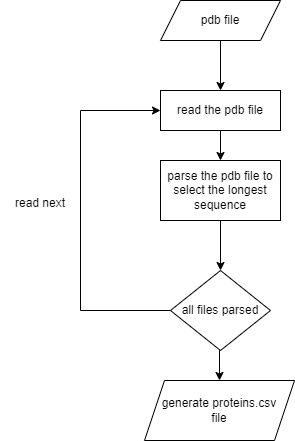
\includegraphics[width=0.4\textwidth]{pdb parser.png} % Replace 'example-image' with the path to your image file
            \caption{PDB file example.}
            \label{fig 4}
        \end{figure}

    \end{itemize} 

    \subsection{drug(ligand) representation}
    the ligand data are provided as \textbf{Structure Data file(SDF)} file format used for representing chemical compounds and their associated data. It is primarily used to store information about molecules, including their structure and various properties, in a structured way.

    the SDF file name is named after the protein ID with which the ligand is paired. consider SDF file \textbf{6M2N\_ligand.sdf} shown in fig \ref{fig 5} where its name does not indicate any information about the ligand but suggests it will be paired with previous protein
    to get information about the ligand itself, it can be open using a text editor e.g. notepad++ and at the end of the file information that identify the ligand can be found e.g. \textbf{chemical formula} and \textbf{Simplified Molecular Input Line Entry System(SMILES)} notation which is is a chemical notation that allows a user to represent a chemical structure in a way that can be used by the computer.
    
    \begin{figure}[h]
        \centering
        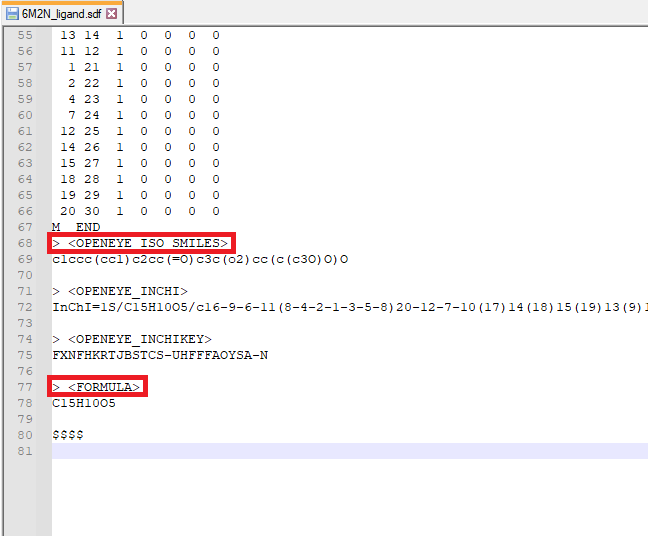
\includegraphics[width=0.7\textwidth]{sdf file.PNG} % Replace 'example-image' with the path to your image file
        \caption{SDF file example.}
        \label{fig 5}
    \end{figure}

    while the chemical formula may not be unique, the SMILES notation is always unique. so it can be used in many websites e.g. the chemspider website\cite{6}  to search for more information about the ligand

    \begin{figure}[h]
        \centering
        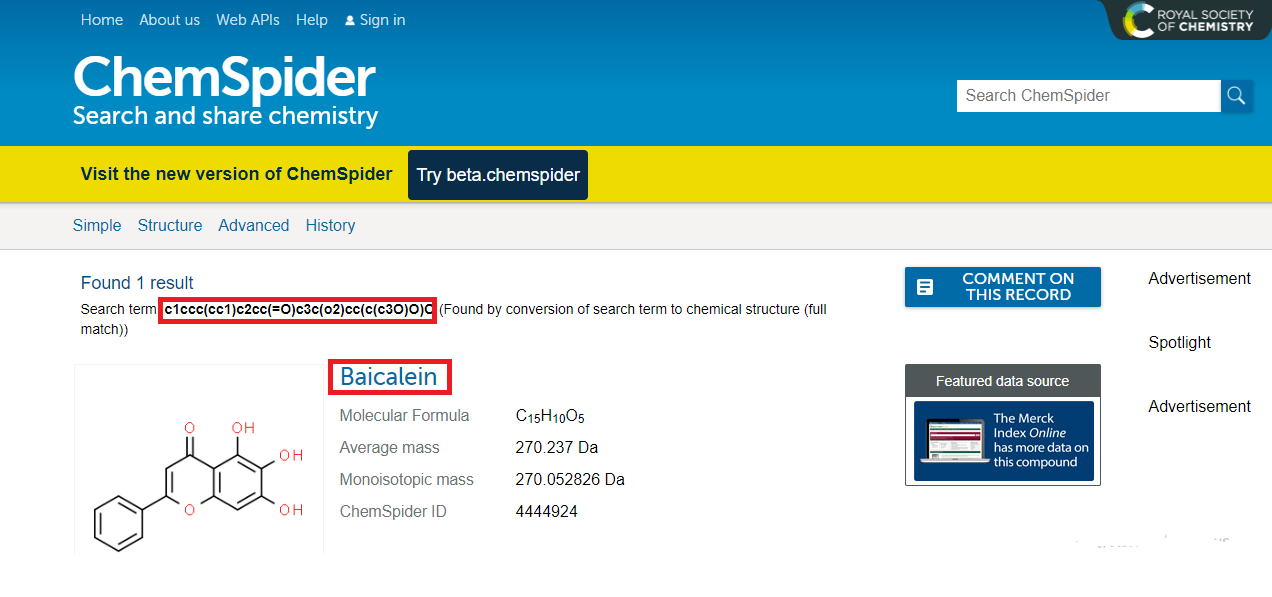
\includegraphics[width=0.9\textwidth]{sdf website.PNG} % Replace 'example-image' with the path to your image file
        \caption{SDF website.}
        \label{fig 6}
    \end{figure}

    An SDF ligand file is read and first the molecule is validated(sanitized) to check if error exist in the structure, if the structure is valid the SMILES notation
    is extracted and appended to valid ligands SDF file else it is excluded and added to invalid ligands SDF file.

    The \textbf{rdkit.Chem} package \cite{7} was used to read the molecule using Chem.SDMolSupplier function, validate it using Chem.SanitizeMol and convert it to SMILES notation
    using function Chem.MolToSmiles

    \begin{itemize}
        \item \textbf{Chem.SDMolSupplier} used to read the molecule.
        \item \textbf{Chem.SanitizeMol} used to validate the molecule             
        \item \textbf{Chem.MolToSmiles} obtain the SMILES notation of the molecule 
    \end{itemize}

    \begin{figure}[h]
        \centering
        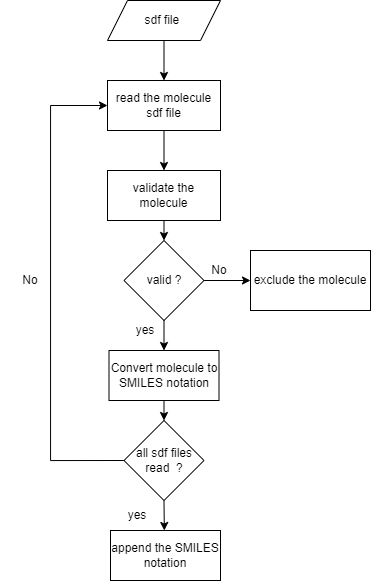
\includegraphics[width=0.5\textwidth]{sdf parser.png} % Replace 'example-image' with the path to your image file
        \caption{SDF workflow.}
        \label{fig 7}
    \end{figure}

    \subsection{affinity representation}
        affinity is the continouos variable that represents the interaction between the ligand and the protein smaller value means less affinity and 
        higher value indicates strong affinity.

        affinity values are provided in csv file linked with protein ID and the protein ID in turn is found in the names of the files of both ligand and the protein

        the following figures explain statistics of the affinity values of the 322 pairs, note that jitter was added to one version of the box plot for the sake of clarity
        
        \begin{figure}[h]
            \centering
            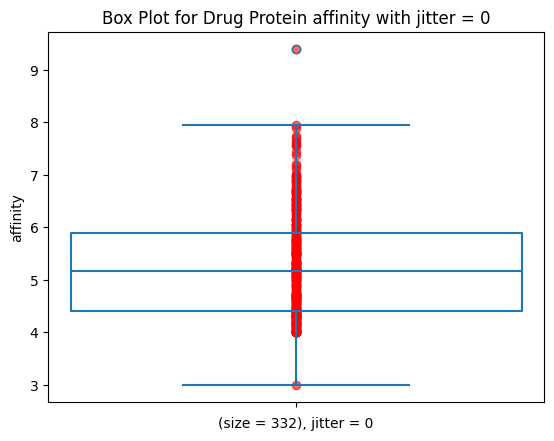
\includegraphics[width=0.5\textwidth]{boxplot1.png} 
            \caption{}
            \label{fig 8}
        \end{figure}
        
        \begin{figure}[h]
            \centering
            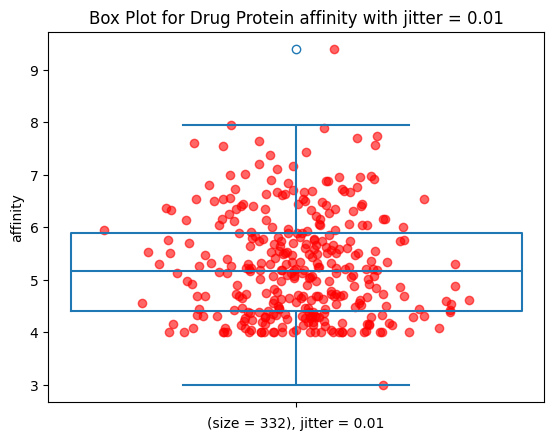
\includegraphics[width=0.5\textwidth]{boxplot2.png}
            \caption{}
            \label{fig 9}
        \end{figure}

        \begin{center}
            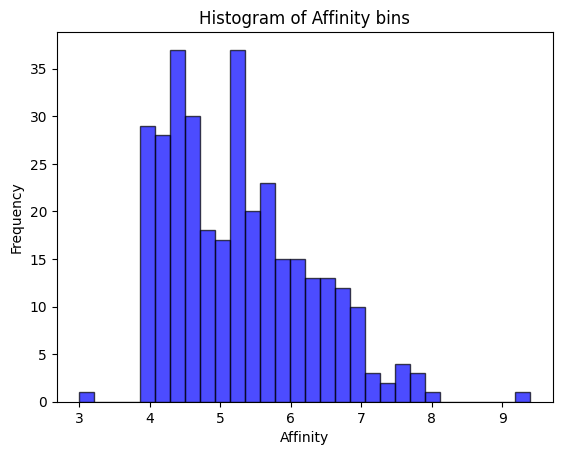
\includegraphics[width=0.5\textwidth]{histogram.png}
        \end{center}

    
            


\section{Network architecture}
    The overall architecture combines the information from the molecular graph and the protein sequence to make a prediction. it is a PyTorch implementation of a Graph Convolutional Network (GCN) based model

    \begin{center}
        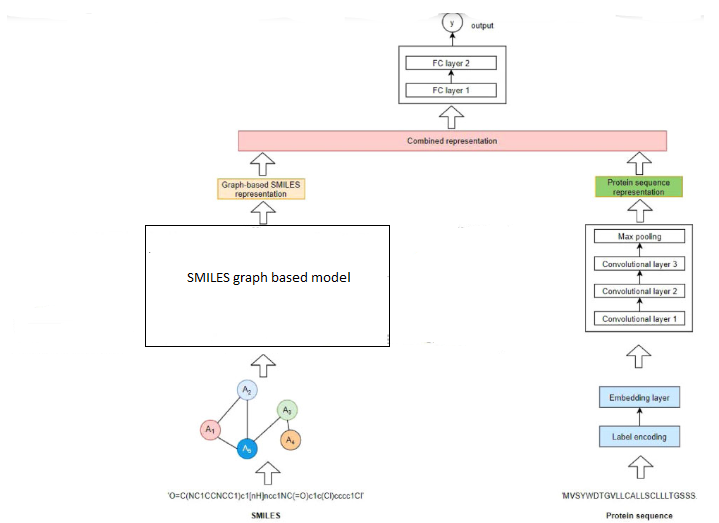
\includegraphics[width=0.8\textwidth]{architecture.PNG}
    \end{center}

    The architecture consists of two main branches where the SMILES graph based branch could be replaced by any of the four SMILES graph branch models :

    \begin{itemize}
        \item \textbf{SMILES graph branch}: operates on the molecular graph representation of the input SMILES. could be any of four models
        \begin{itemize}
            \item \textbf{GCN model} 
                \begin{enumerate}
                    \item It uses three GCN layers (GCNConv) to extract features from the graph. The number of filters and feature dimensions are increased in the subsequent layers.
                    \item After the GCN layers, the extracted features are passed through two fully connected layers (fc\_g1 and fc\_g2) to obtain a fixed-size output representation.
                \end{enumerate}

                \begin{center}
                    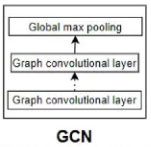
\includegraphics[width=0.3\textwidth]{GCN_model.PNG}
                \end{center}

            \item \textbf{GAT model}
                \begin{enumerate}
                    \item The model starts with two GAT layers, gcn1 and gcn2, which operate on the input graph data.
                    \item The first GAT layer, gcn1, takes the initial node features (num\_features\_xd) and outputs a representation with 10 heads, effectively increasing the feature dimensionality by a factor of 10.
                    \item The second GAT layer, gcn2, then reduces the feature dimensionality to output\_dim.
                    \item After the GAT layers, a fully connected layer fc\_g1 is applied to the output of the second GAT layer.
                \end{enumerate}

                \begin{center}
                    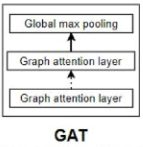
\includegraphics[width=0.3\textwidth]{GAT_model.PNG}
                \end{center}

            \item \textbf{GIN model}
                \begin{enumerate}
                    \item The model has 5 GINConv layers, each with a sequential neural network (nn1, nn2, ..., nn5) that consists of a Linear layer, a ReLU activation, and another Linear layer.
                    \item Each GINConv layer is followed by a BatchNorm1d layer to normalize the output.
                \end{enumerate}

                \begin{center}
                    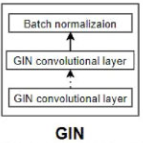
\includegraphics[width=0.3\textwidth]{GIN_model.PNG}
                \end{center}

            \item \textbf{GAT-GCN model}
                \begin{enumerate}
                    \item The first layer is a GATConv layer, which implements the Graph Attention Network mechanism. It takes the input node features (num\_features\_xd) and outputs features with the same dimensionality, but with 10 attention heads.
                    \item The second layer is a GCNConv layer, which applies a standard Graph Convolutional Network operation. It takes the concatenated output of the previous GAT layer (10 times the original number of features) and outputs the same number of features.
                \end{enumerate}

                \begin{center}
                    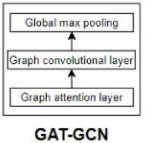
\includegraphics[width=0.3\textwidth]{GAT_GCN.PNG}
                \end{center}

        \end{itemize} 
        \item \textbf{Protein sequence branch}: operates on the protein sequence input, which is represented as a sequence of integer indices of characters representing amino acids.
            \begin{enumerate}
                \item The protein sequence is passed through an embedding layer (embedding\_xt) to convert the integer indices into a dense vector representation.
                \item The embedded sequence is then passed through a 1D convolutional layer (conv\_xt\_1) to extract features from the protein sequence.
                \item The convolutional features are flattened and passed through a fully connected layer (fc1\_xt) to obtain a fixed size output representation.
            \end{enumerate} 
    \end{itemize} 
    After obtaining the output representations from the two branches, the model concatenates them and passes the combined features through two more fully connected layers (fc1 and fc2) to produce the final output.

The model uses ReLU activations, dropout for regularization, and global max pooling (gmp) to aggregate the graph-level features.

    \subsection{GCN-based graph representation learning}
        The GCNNet class is a neural network model designed for processing two types of input data: molecular graphs (represented by SMILES strings) and protein sequences. This model uses a combination of Graph Convolutional Networks (GCNs) for the molecular graphs and 1D Convolutional Networks (Conv1D) for the protein sequences.

\section{Results}
    \subsection{train and test GCN model on the URV dataset with k folds = 10}
    Apply k-folding with k = 10 to get 10 different combinations of train and test patterns for URV dataset using GCN model gives the following error evolutions and real predicted affinity
    
    the mean MSE is 0.84
    
    the mean standard deviation is 0.97
    \begin{center}
        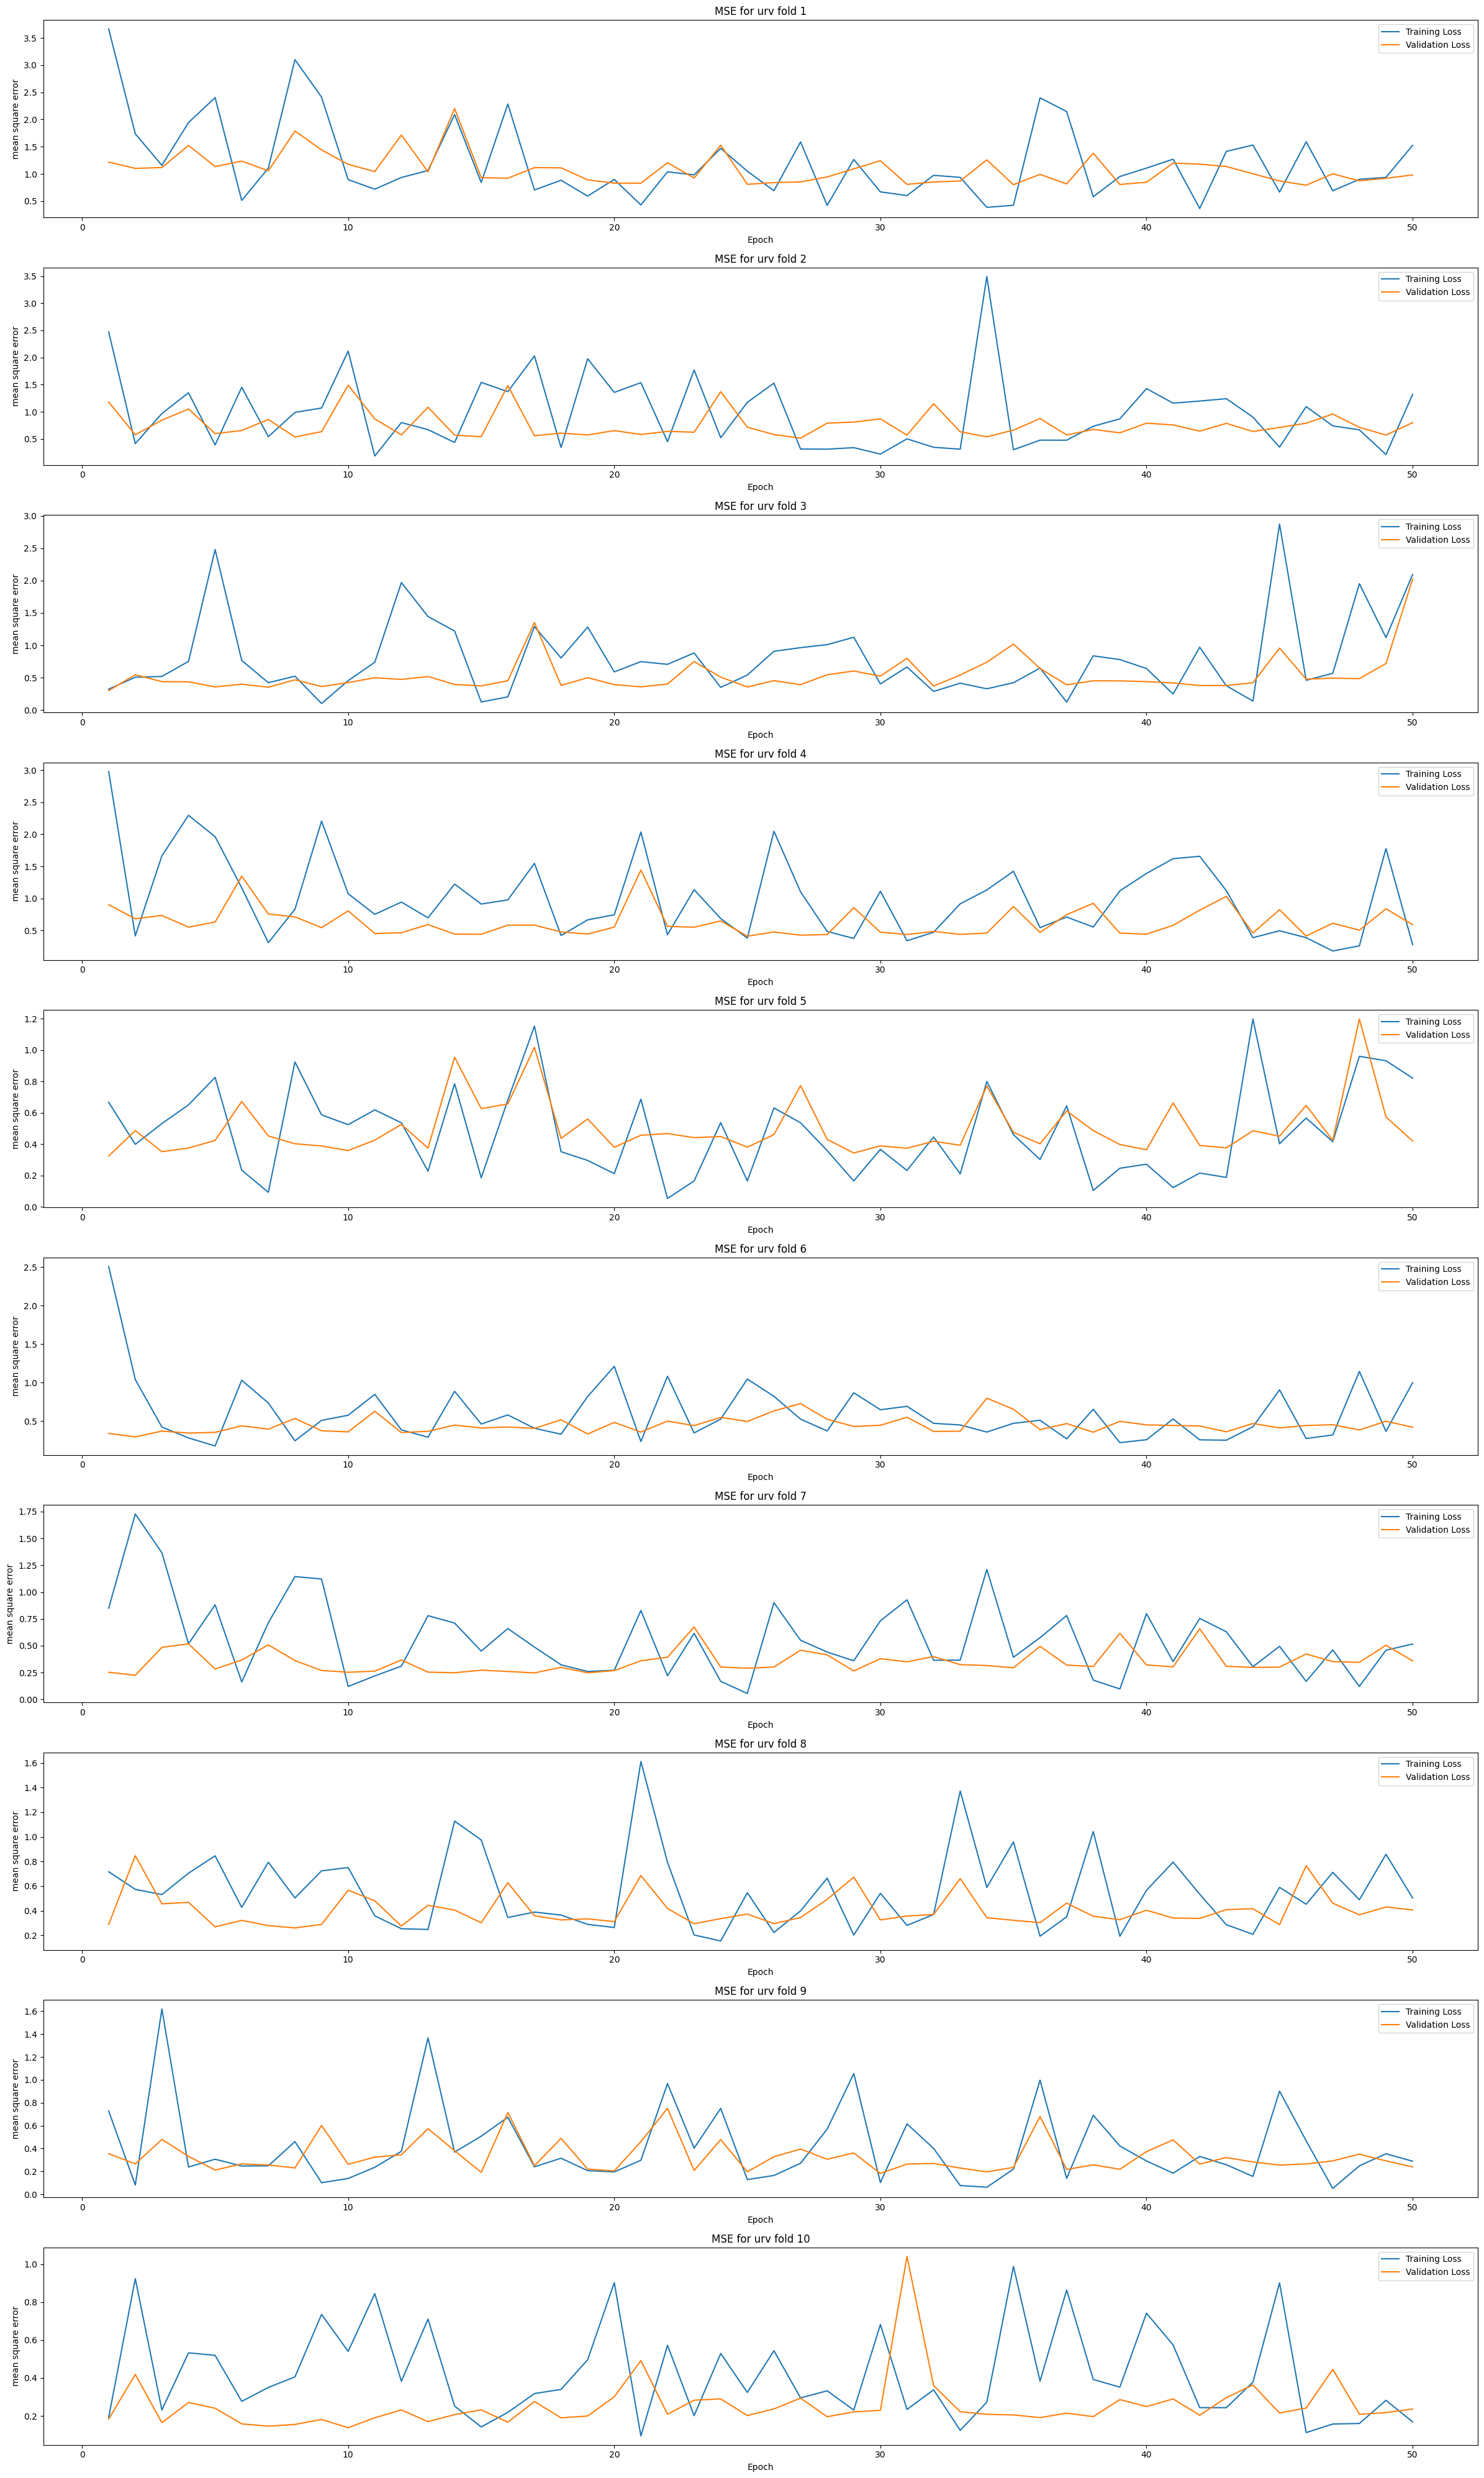
\includegraphics[width=0.9\textwidth]{GCN_folds10errors.png}
    \end{center}

    \begin{center}
        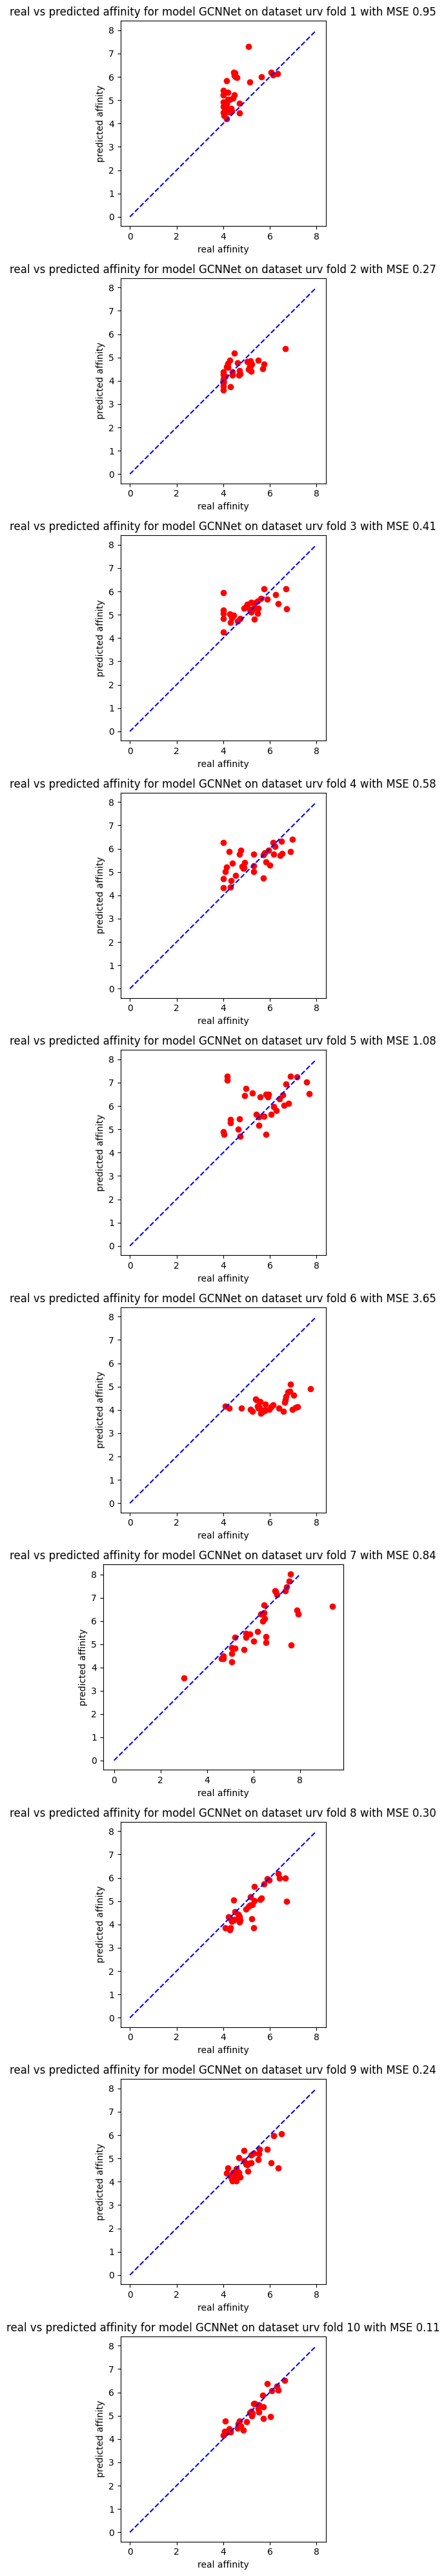
\includegraphics[width=0.25\textwidth]{GCN_folds10predictions.png}
    \end{center}

    \subsection{train and test GAT model on the URV dataset with k folds = 10}
    Apply k-folding with k = 10 to get 10 different combinations of train and test patterns for URV dataset using GAT model gives the following error evolutions and real predicted affinity
    
    the mean MSE is 1.50

    the mean standard deviation is 1.13

    \begin{center}
        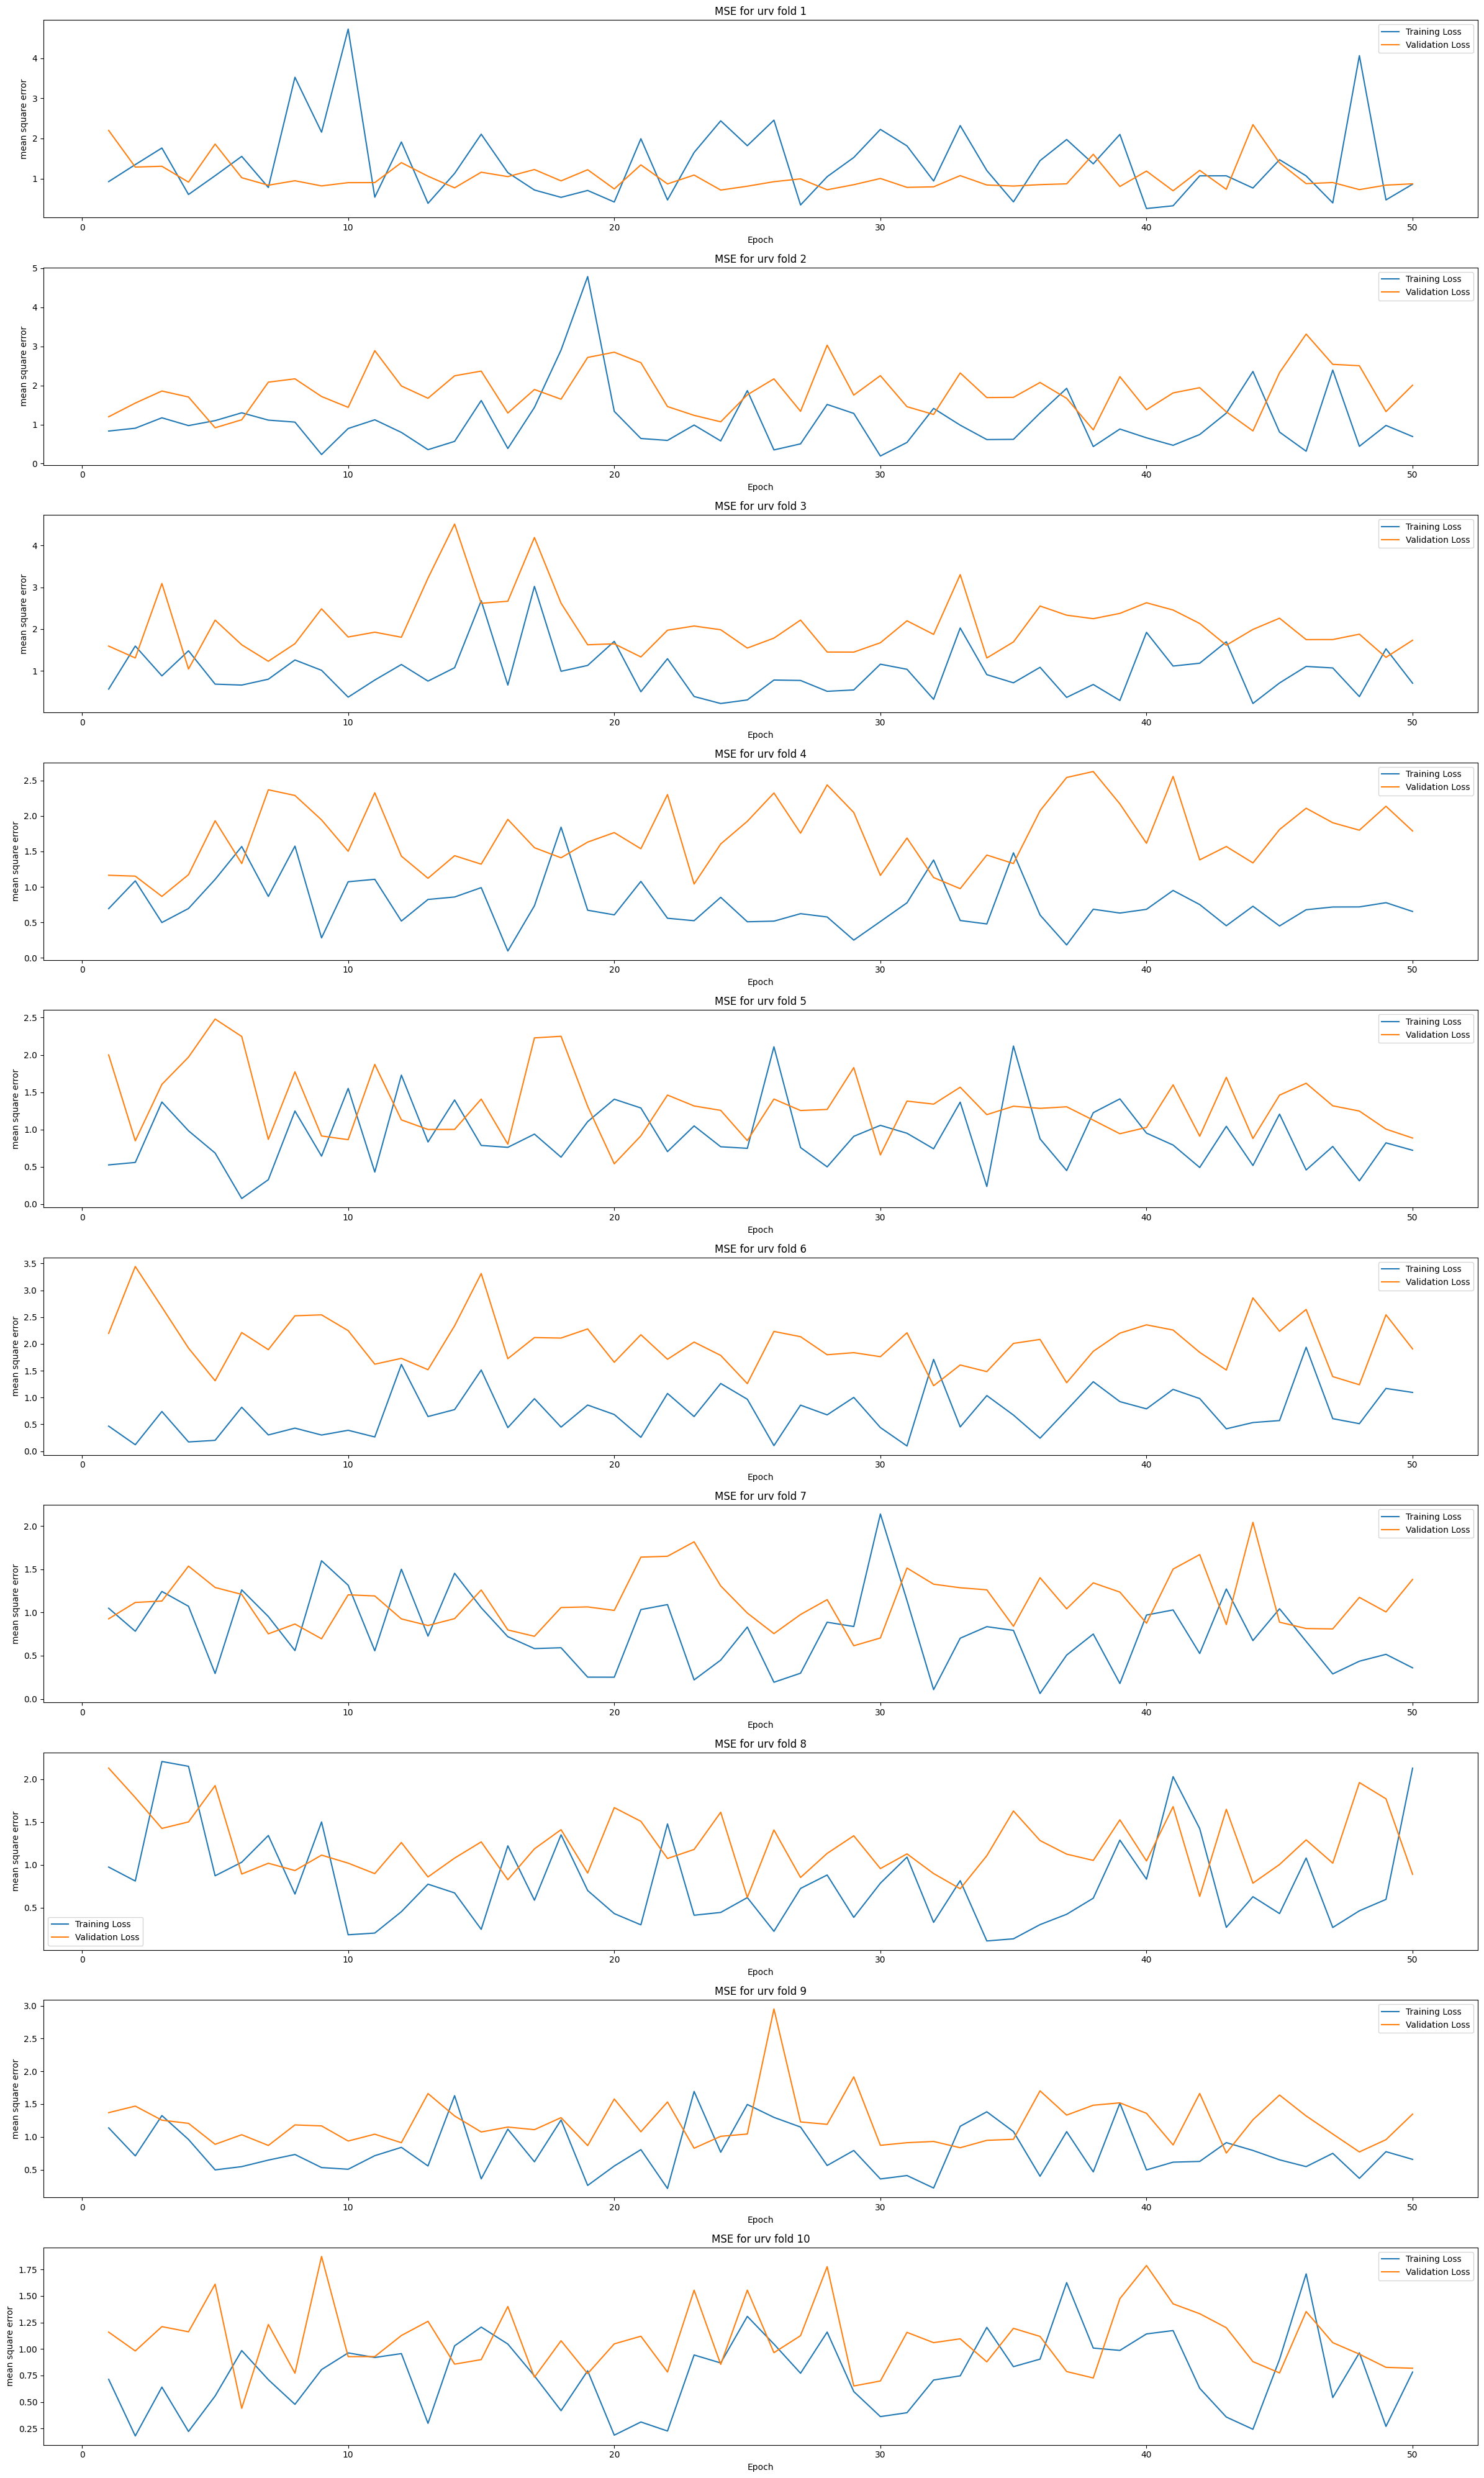
\includegraphics[width=0.9\textwidth]{GAT_folds10errors.png}
    \end{center}

    \begin{center}
        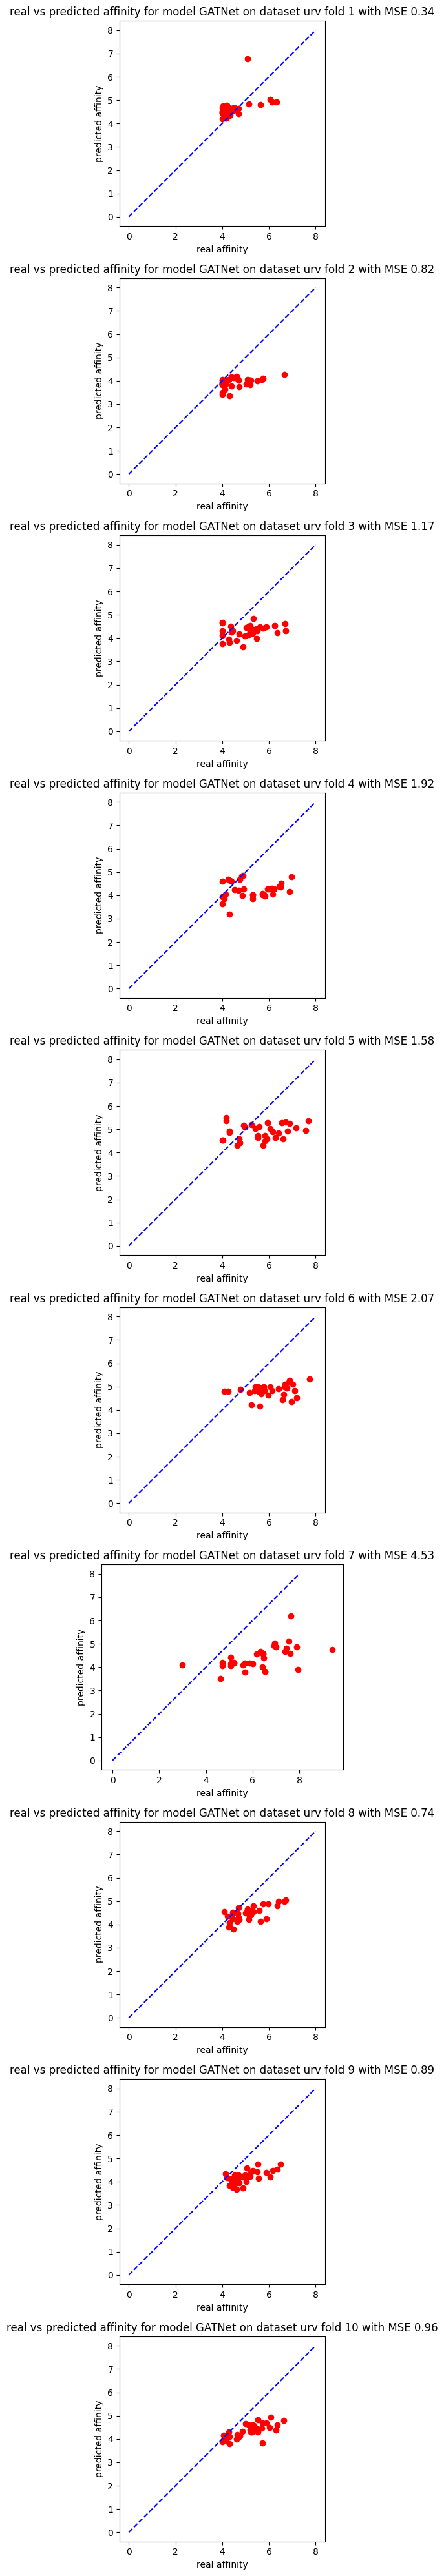
\includegraphics[width=0.25\textwidth]{GAT_folds10predictions.png}
    \end{center}

    \subsection{train and test GATGCN model on the URV dataset with k folds = 10}
    Apply k-folding with k = 10 to get 10 different combinations of train and test patterns for URV dataset using GATGCN model gives the following error evolutions and real predicted affinity
    
    the mean MSE is 0.44

    the mean standard deviation is 0.24

    \begin{center}
        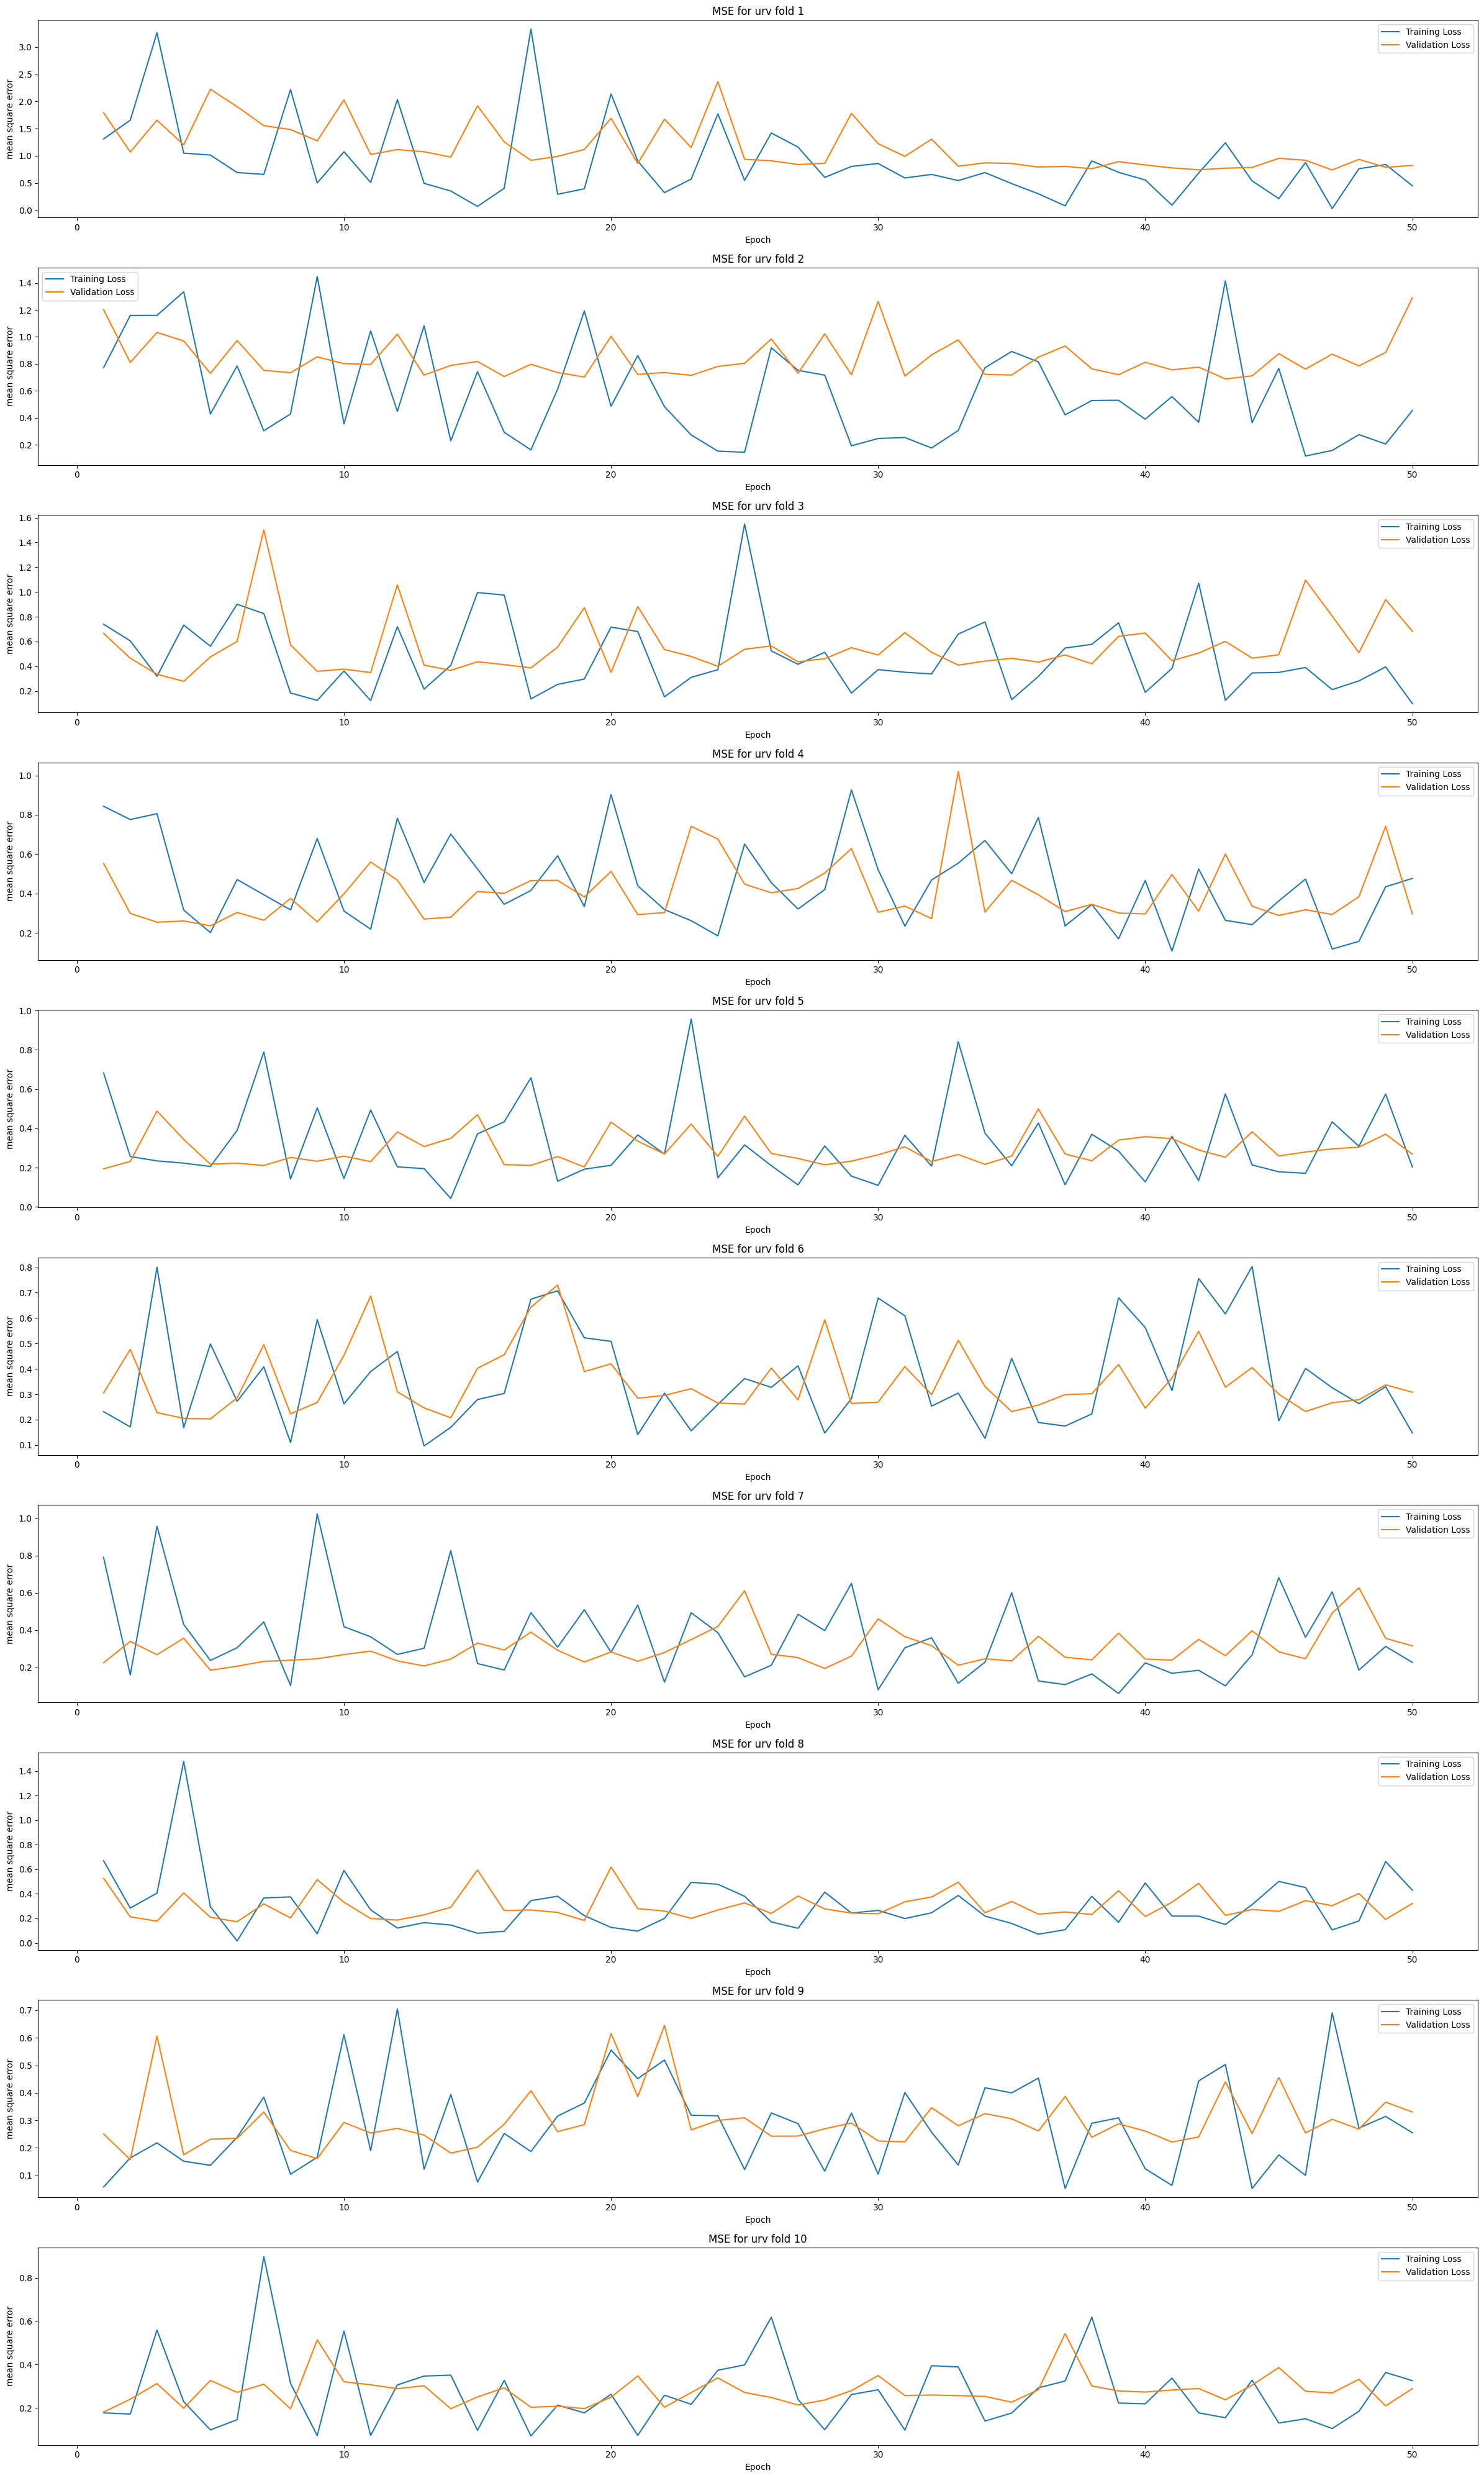
\includegraphics[width=0.9\textwidth]{GATGCN_folds10errors.png}
    \end{center}

    \begin{center}
        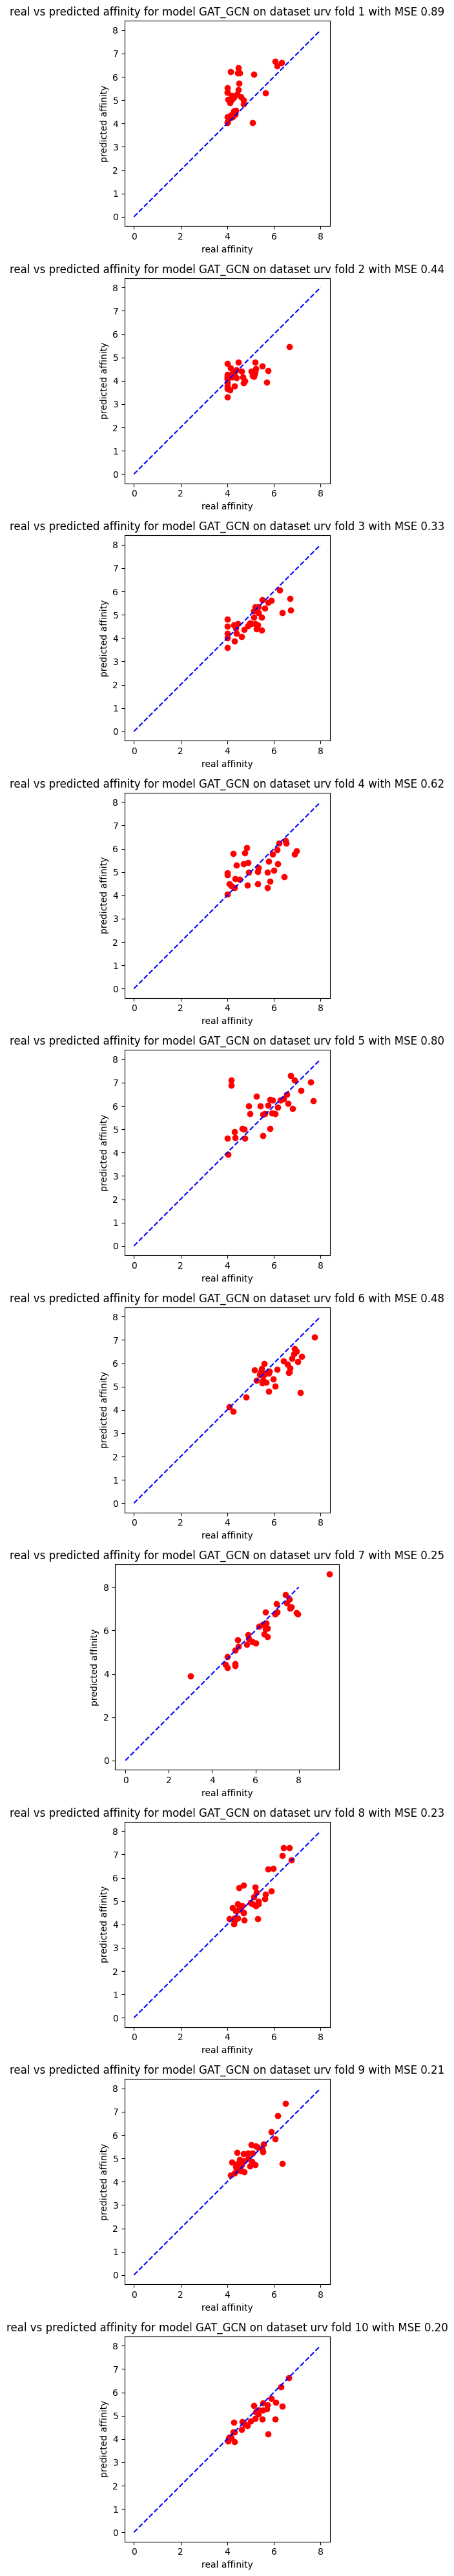
\includegraphics[width=0.25\textwidth]{GATGCN_folds10predictions.png}
    \end{center}

    \subsection{train and test GINCONV model on the URV dataset with k folds = 10}
    Apply k-folding with k = 10 to get 10 different combinations of train and test patterns for URV dataset using GINCONV model gives the following error evolutions and real predicted affinity
    
    the mean MSE is 0.76

    the mean standard deviation is 0.56

    \begin{center}
        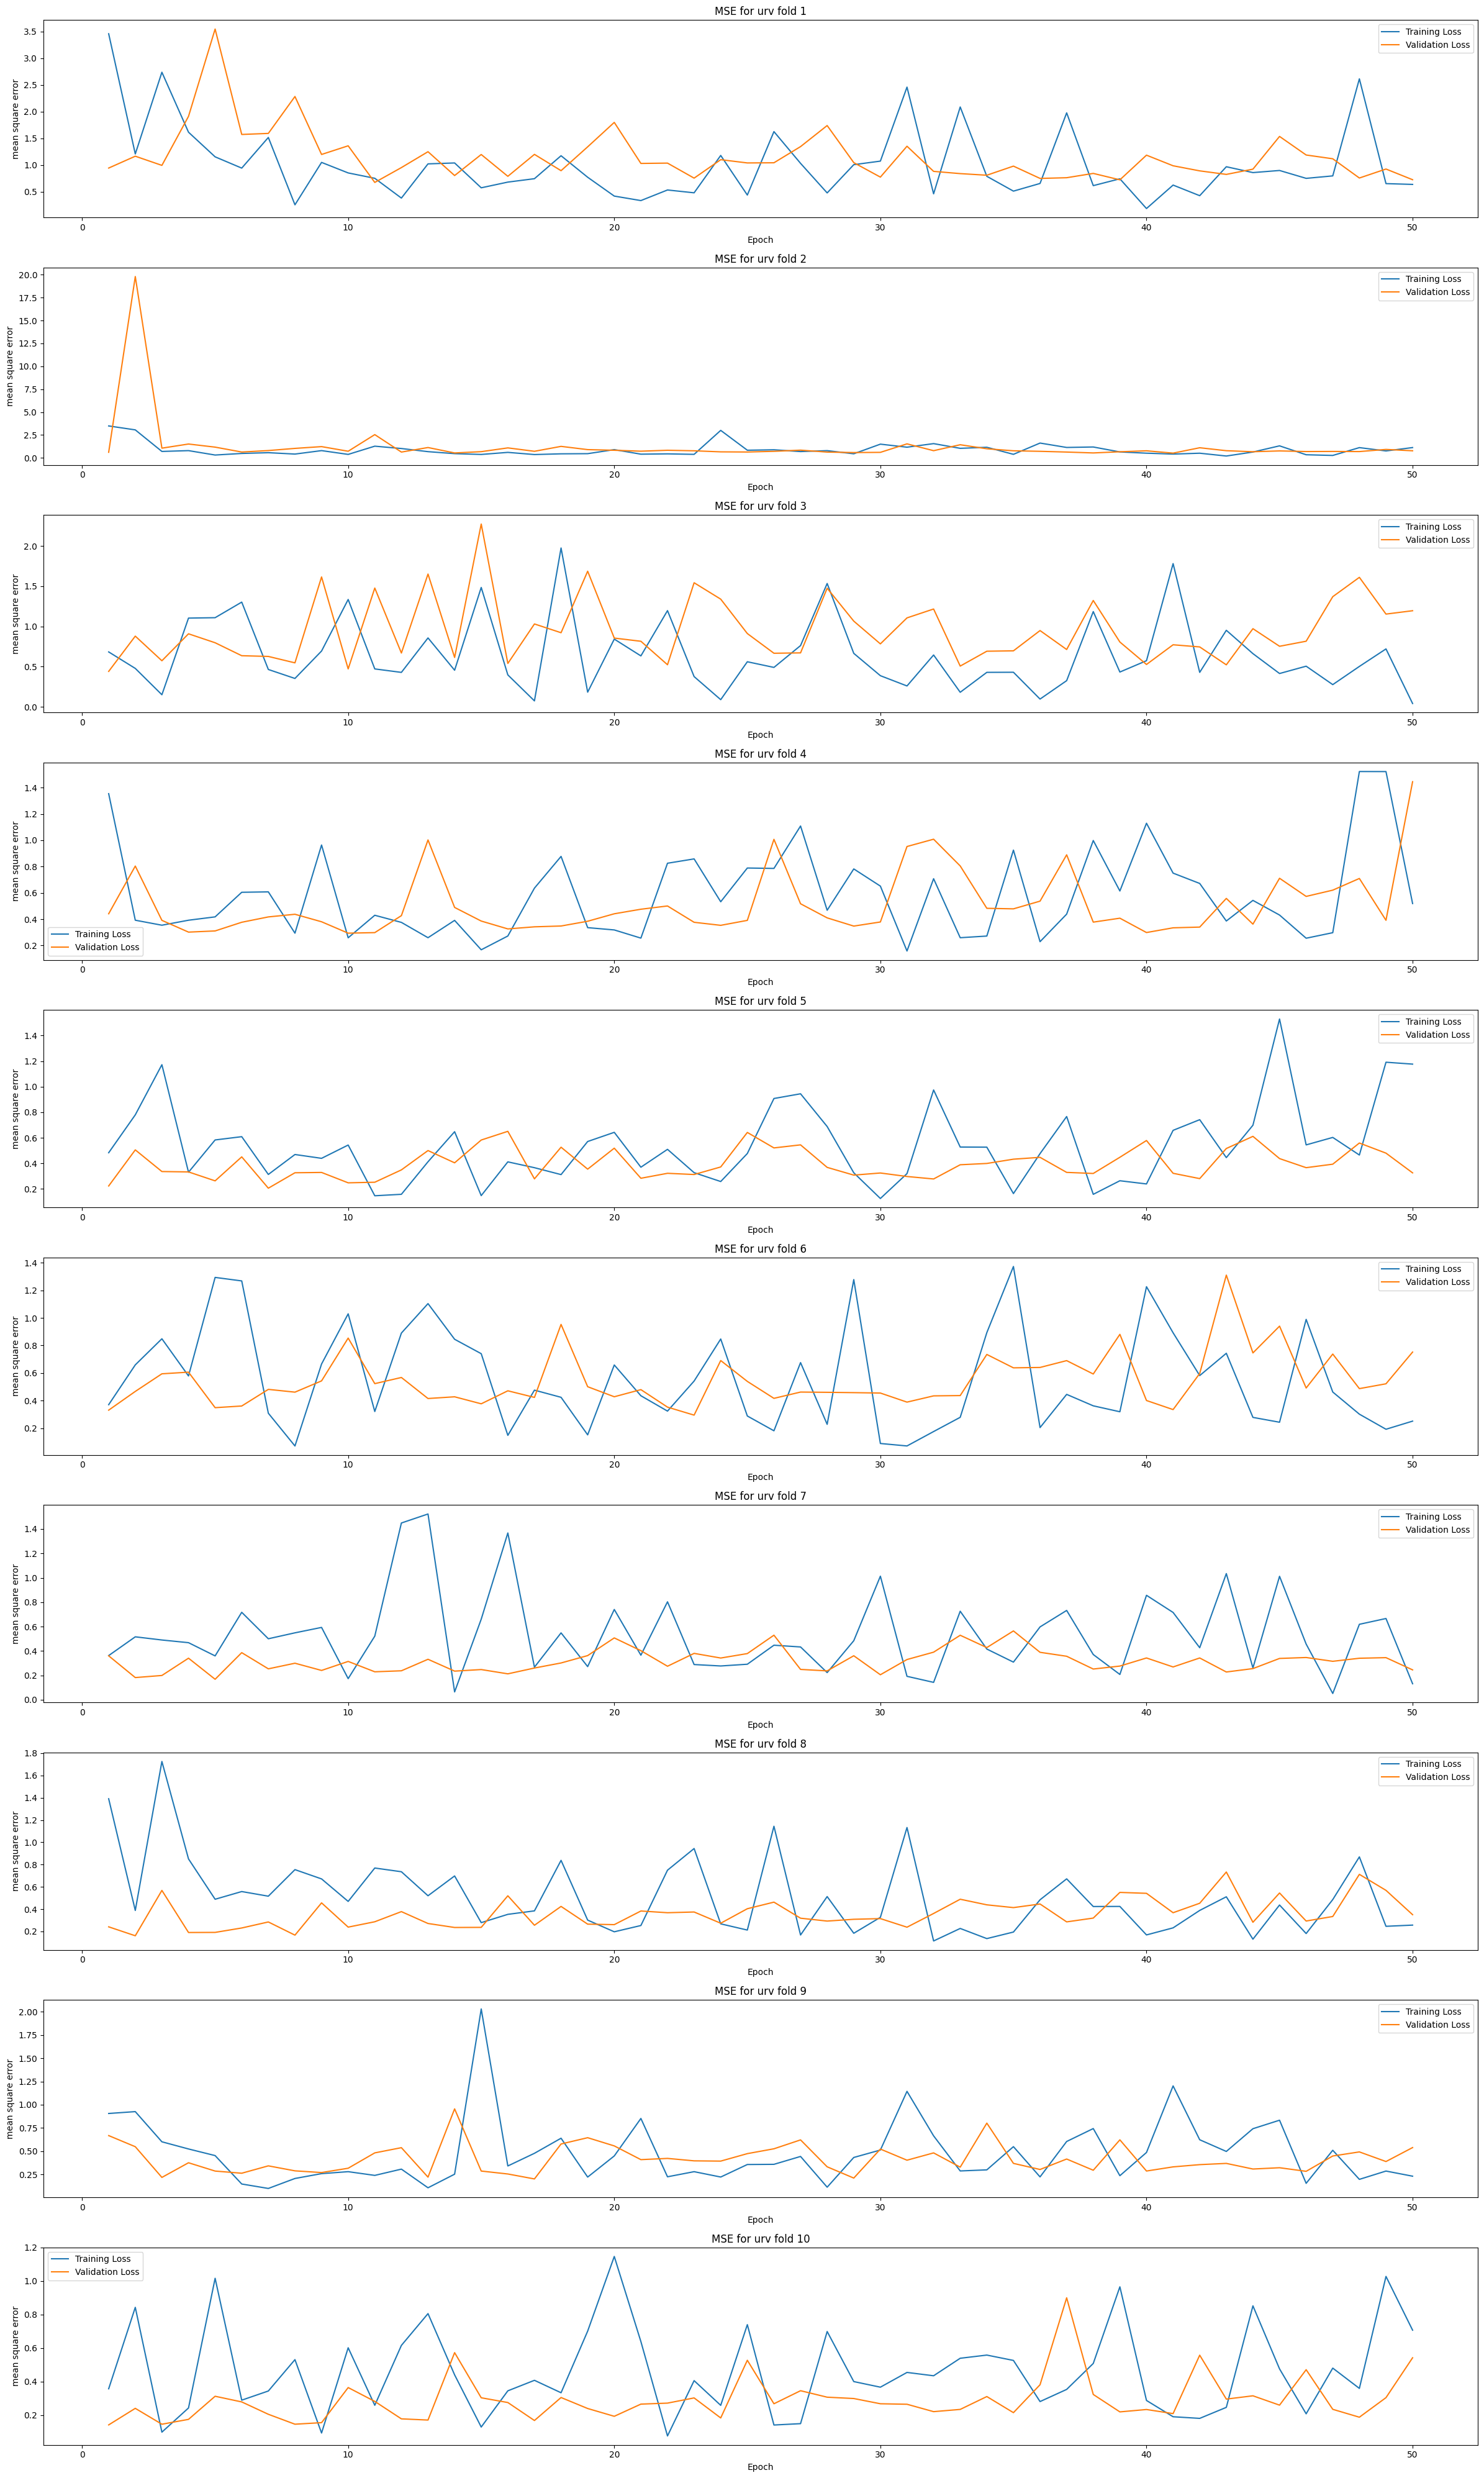
\includegraphics[width=0.9\textwidth]{GINCONV_folds10errors.png}
    \end{center}

    \begin{center}
        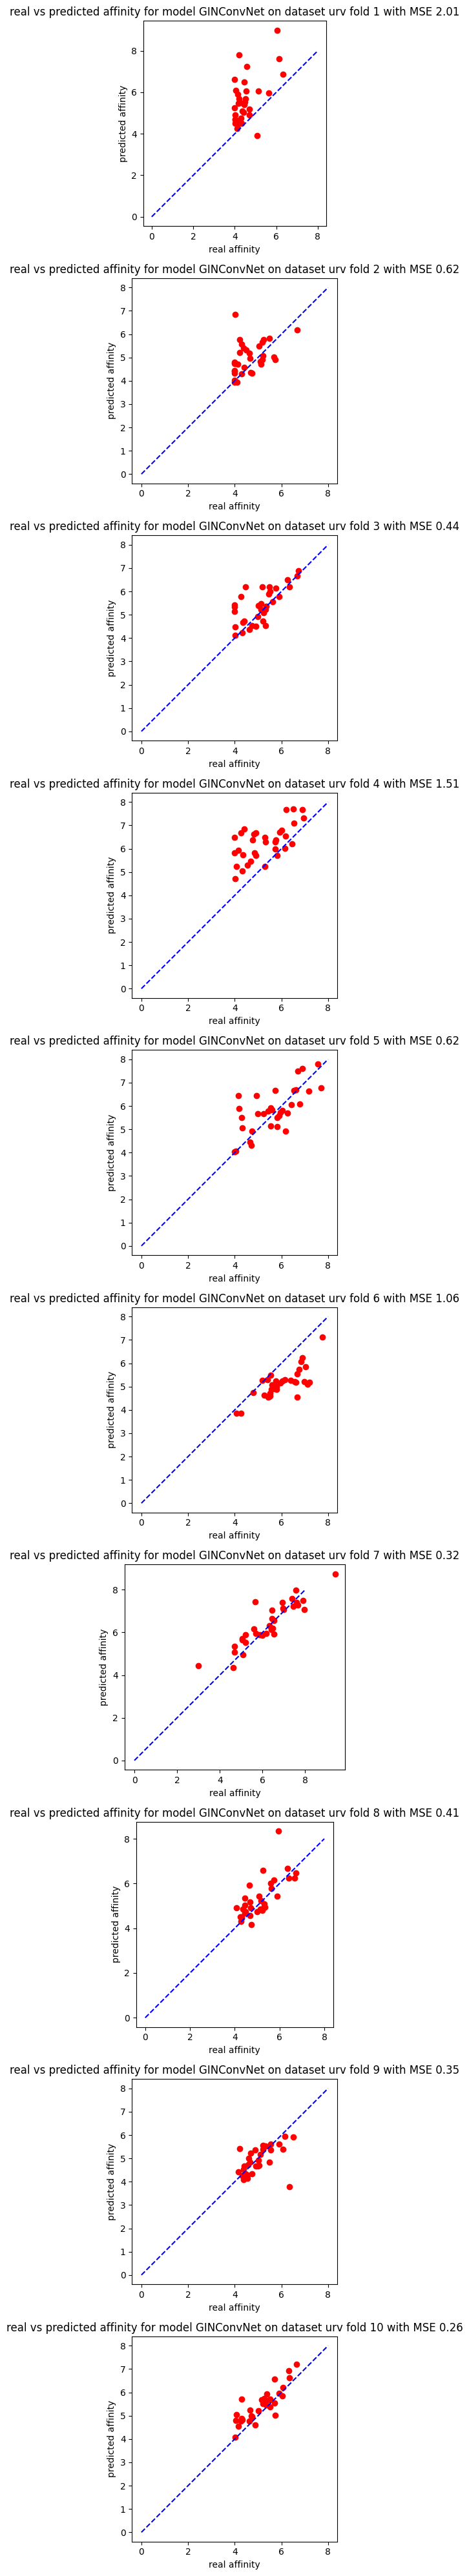
\includegraphics[width=0.25\textwidth]{GINCONV_folds10predictions.png}
    \end{center}
%\addcontentsline{toc}{section}{Bibliography} % Add Bibliography to TOC
%\printbibliography 
\begin{thebibliography}{3}

\bibitem{1}
    [Thin et al.] Thin Nguyen;  Hang Le; Thomas P. Quinn; Tri Nguyen; Thuc Duy Le; and
    Svetha Venkatesh, "GraphDTA: predicting drug–target binding affinity with
    graph neural networks",
    \\Journal Bioinformatics, Volume 37, Issue 8, March 2021, Pages 1140–1147
    \\Available at
    \url{https://academic.oup.com/bioinformatics/article/37/8/1140/5942970}.

\bibitem{2}
    Related data, pre-trained models and source code in \cite{1} are publicly available at \url{https://github.com/thinng/GraphDTA}.

\bibitem{3}
    the repository forked from \cite{2} to perform experiments in this thesis available at \url{https://github.com/YoussefEzz/GraphDTA_forked}.
\bibitem{4}
PDB website: \url{https://www.rcsb.org/}.

\bibitem{5}
Bio.PDB Biopython module: \url{https://biopython.org/wiki/The_Biopython_Structural_Bioinformatics_FAQ}.

\bibitem{6}
chemspider website: \url{https://www.chemspider.com/}.

\bibitem{7}
chemspider website: \url{https://www.rdkit.org/docs/source/rdkit.Chem.html}.

\end{thebibliography}

\end{document}
